\documentclass[aspectratio=169, table]{beamer}
\usepackage[utf8]{inputenc}
\usepackage[T1]{fontenc}
\usepackage{graphicx}
\usepackage{fontspec}
\usepackage{xcolor}
\usepackage{tcolorbox}
\usepackage{listings} % Add the listings package
\usepackage{hyperref} % Add the hyperref package

\lstdefinelanguage{JavaScript}{
    keywords={function, var, let, const, if, else, for, while, return, true, false},
    keywordstyle=\color{blue}\bfseries,
    ndkeywords={class, export, boolean, throw, implements, import, this},
    ndkeywordstyle=\color{orange}\bfseries,
    identifierstyle=\color{black},
    sensitive=false,
    comment=[l]{//},
    morecomment=[s]{/*}{*/},
    commentstyle=\color{gray}\ttfamily,
    stringstyle=\color{green}\ttfamily,
}

\lstset{
    breaklines=true,
    language=JavaScript,
    % ... (other style settings)
}

\lstdefinelanguage{PHP}{
    keywords={class, function, echo, if, else, foreach, for, while, return},
    keywordstyle=\color{blue}\bfseries,
    ndkeywords={public, private, protected, static},
    ndkeywordstyle=\color{purple}\bfseries,
    identifierstyle=\color{black},
    sensitive=false,
    comment=[l]{//},
    morecomment=[s]{/*}{*/},
    commentstyle=\color{gray}\ttfamily,
    stringstyle=\color{green}\ttfamily,
}

\lstset{
    breaklines=true,
    language=PHP,
    % ... (other style settings)
}

\setsansfont[
  ItalicFont=fonts/TitilliumWeb-Italic.ttf,
  BoldFont=fonts/TitilliumWeb-Bold.ttf,
  BoldItalicFont=fonts/TitilliumWeb-BoldItalic.ttf,
]{TitilliumWeb-Regular.ttf}

\subtitle{IF140303 Web-based Application Development}
\title{\Huge {\textbf{12: \\Database}}}
\date[Serial]{\scriptsize {PRU/SPMI/FR-BM-18/0222}}
\author[Pradita]{\small {\textbf{PRADITA UNIVERSITY}}}

\usetheme{Pradita}

\begin{document}
\begin{frame}
    \titlepage
\end{frame}

\begin{frame}{Goals - Database}
    \vskip1cm
    \begin{itemize}
        \item Understand the fundamentals of databases and their role in web development.
        \item Exposure on relational database management systems (DBMS).
%        \item Gain insight into the use of SQL (Structured Query Language) for database interactions.
        \item Learn about creating, reading, updating, and deleting (CRUD) operations on databases.
        \item Explore the concept of database migrations for version control and collaboration.
%        \item Understand the significance of database normalization for efficient data storage.
        \item Gain hands-on experience by integrating databases with web applications.
    \end{itemize}
\end{frame}

\begin{frame}{Introduction to Database}
    \vskip1cm
    \begin{itemize}
        \item A database is a structured collection of data that is organized and managed to provide efficient retrieval and manipulation.
        \item Databases play a crucial role in web development by providing a way to store, manage, and retrieve data for applications.
        \item Databases are used to store various types of information, including user data, product information, orders, and more.
        \item Web applications often require efficient and reliable data storage to provide a seamless user experience.
        \item Different types of databases exist, such as relational databases, NoSQL databases, and in-memory databases.
        \item The choice of a database type depends on factors like the nature of data, scalability, and performance requirements.
    \end{itemize}
\end{frame}

\begin{frame}{Migration Laravel}
    \vskip1cm
    \begin{itemize}
        \item Migration is a version control for the database schema
        \item In Laravel Project CMD: php artisan make:migration create\_converter\_table
        \item Running Migration: php artisan migrate 
        \item Refresh: php artisan migrate:refresh
        \item Rollback: php artisan migrate:rollback
        \item Code in Next Slide
    \end{itemize}
\end{frame}

\begin{frame}[fragile]
 \frametitle{Migration Laravel}
 \vskip1cm
 \begin{center}
  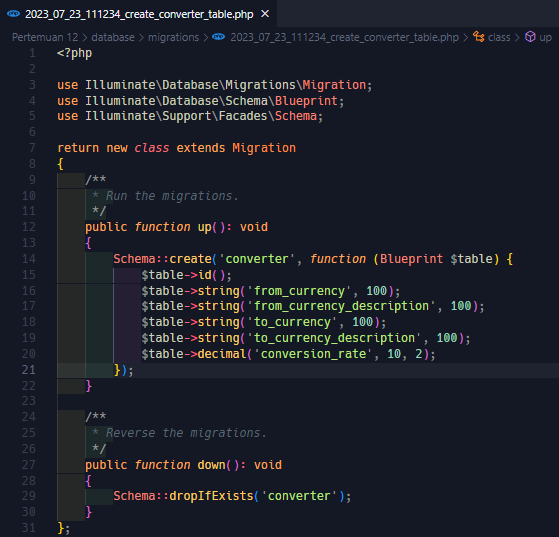
\includegraphics[width=0.6\textwidth]{classFiles/pertemuan-12-migrate.png}
 \end{center}
\end{frame}

\begin{frame}{Seeder Laravel}
    \vskip1cm
    \begin{itemize}
        \item Seeder allows you to easily populate your database with sample/default data.
        \item In Laravel Project CMD: php artisan make:seeder ConverterSeeder
        \item Runing the seeder: php artisan db:seed --class=ConverterSeeder
        \item Code is in the next slide
    \end{itemize}
\end{frame}

\begin{frame}[fragile]
 \frametitle{Seeder Laravel}
 \vskip1cm
 \begin{center}
  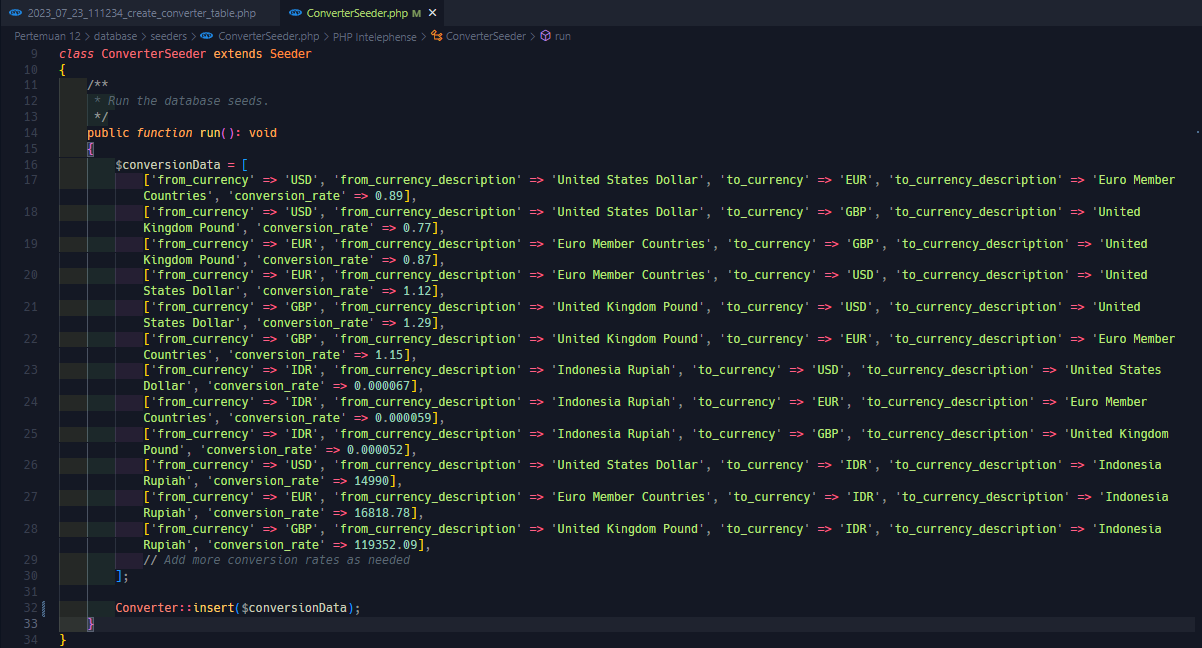
\includegraphics[width=0.6\textwidth]{classFiles/pertemuan-12-seeder.png}
 \end{center}
\end{frame}

\begin{frame}{Models Laravel}
    \vskip1cm
    \begin{itemize}
        \item Models provide an abstraction layer that simplifies database interactions and promotes good coding practices.
        \item In Laravel Project CMD: php artisan make:model Converter
        \item Change the name of the Old Converter model to Converter\_.php or remove it
        \item Code is in the next slide
    \end{itemize}
\end{frame}

\begin{frame}[fragile]
 \frametitle{Model Laravel}
 \vskip1cm
 \begin{center}
  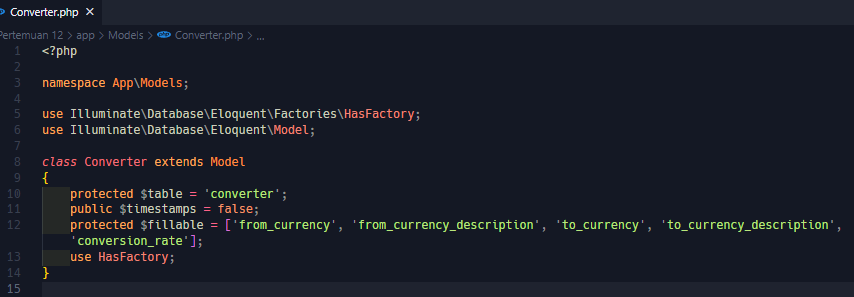
\includegraphics[width=0.6\textwidth]{classFiles/pertemuan-12-model.png}
 \end{center}
\end{frame}

\begin{frame}{Views Laravel}
    \vskip1cm
    \begin{itemize}
        \item Create add-converter.blade.php, edit-converter.blade.php
        \item 
    \end{itemize}
\end{frame}

\begin{frame}[fragile]
 \frametitle{add-converter.blade.php Part 1}
 \vskip1cm
 \begin{center}
  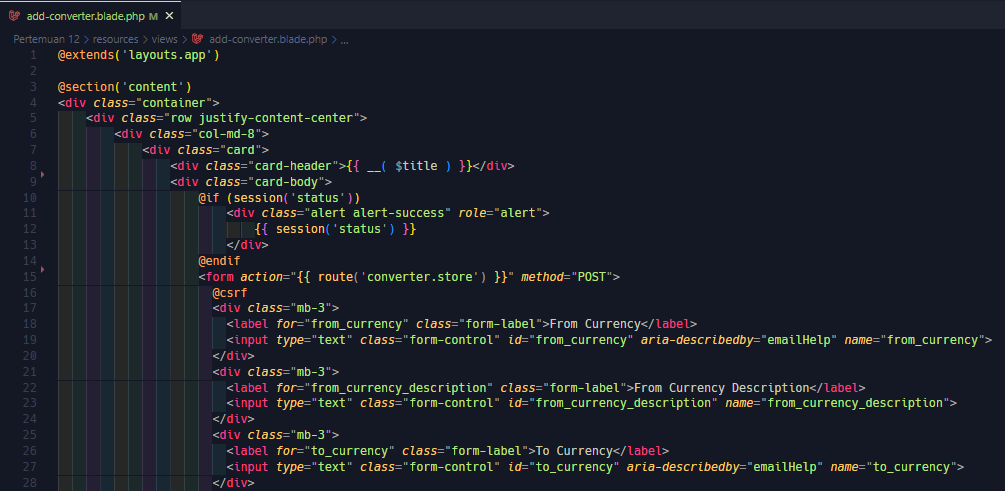
\includegraphics[width=0.6\textwidth]{classFiles/pertemuan-12-view-part-1.png}
 \end{center}
\end{frame}

\begin{frame}[fragile]
 \frametitle{add-converter.blade.php Part 2}
 \vskip1cm
 \begin{center}
  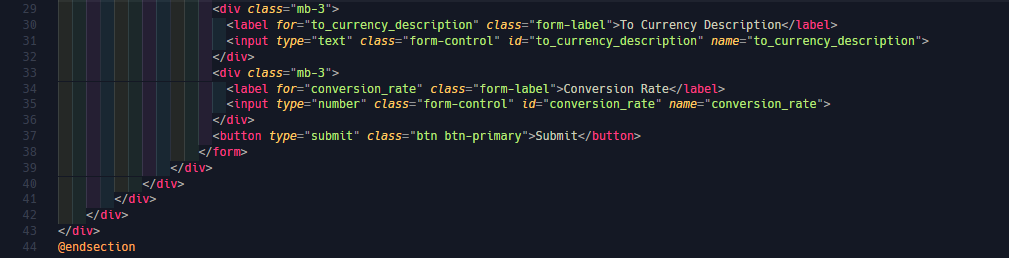
\includegraphics[width=0.6\textwidth]{classFiles/pertemuan-12-view-part-2.png}
 \end{center}
\end{frame}

\begin{frame}[fragile]
 \frametitle{edit-converter.blade.php Part 1}
 \vskip1cm
 \begin{center}
  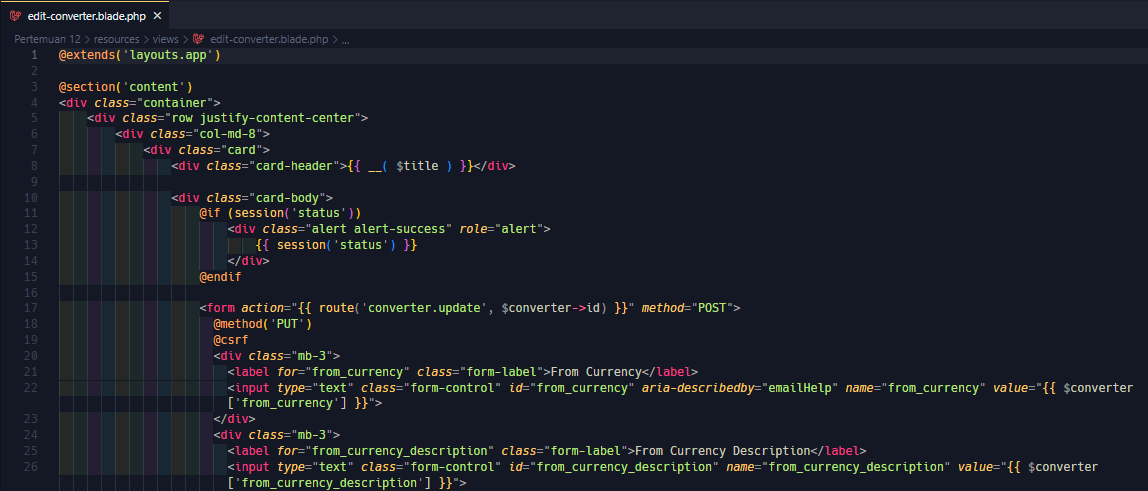
\includegraphics[width=0.6\textwidth]{classFiles/pertemuan-12-view-part-3.png}
 \end{center}
\end{frame}

\begin{frame}[fragile]
 \frametitle{edit-converter.blade.php Part 2}
 \vskip1cm
 \begin{center}
  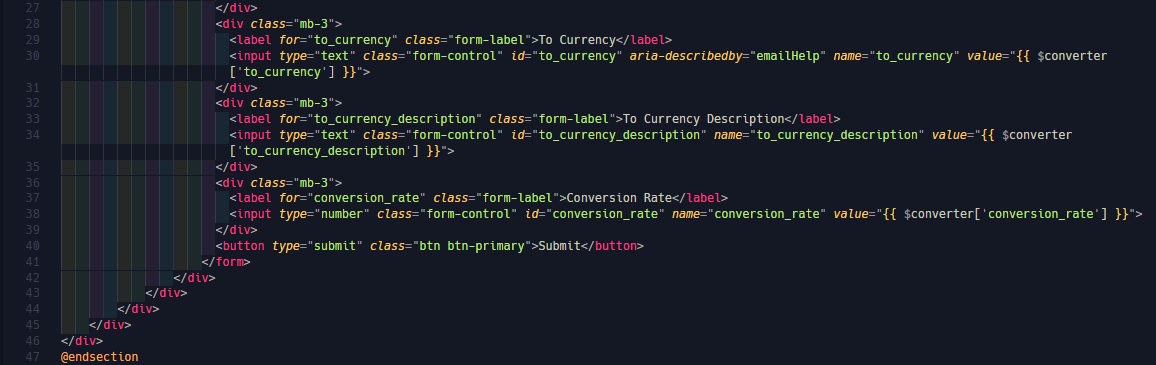
\includegraphics[width=0.6\textwidth]{classFiles/pertemuan-12-view-part-4.png}
 \end{center}
\end{frame}

\begin{frame}[fragile]
 \frametitle{ConverterController.php Part 1}
 \vskip1cm
 \begin{center}
  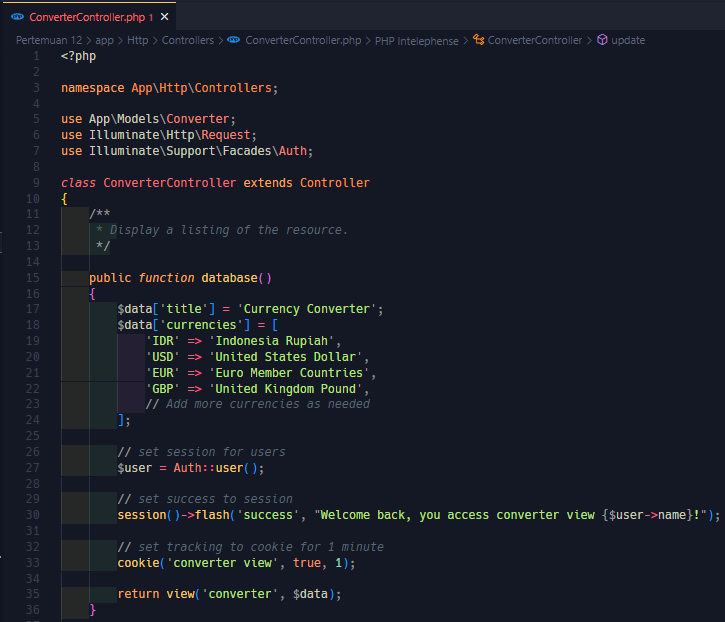
\includegraphics[width=0.6\textwidth]{classFiles/pertemuan-12-controller-part-1.png}
 \end{center}
\end{frame}

\begin{frame}[fragile]
 \frametitle{ConverterController.php Part 2}
 \vskip1cm
 \begin{center}
  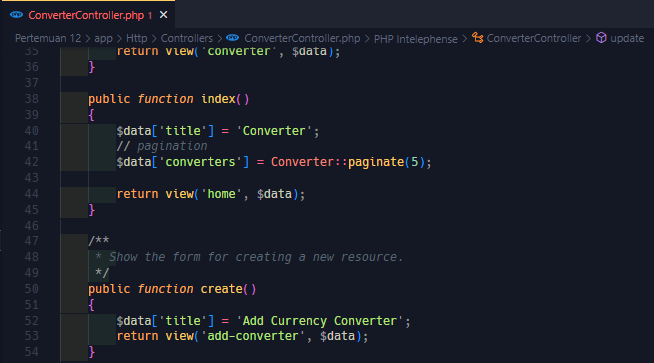
\includegraphics[width=0.6\textwidth]{classFiles/pertemuan-12-controller-part-2.png}
 \end{center}
\end{frame}

\begin{frame}[fragile]
 \frametitle{ConverterController.php Part 3}
 \vskip1cm
 \begin{center}
  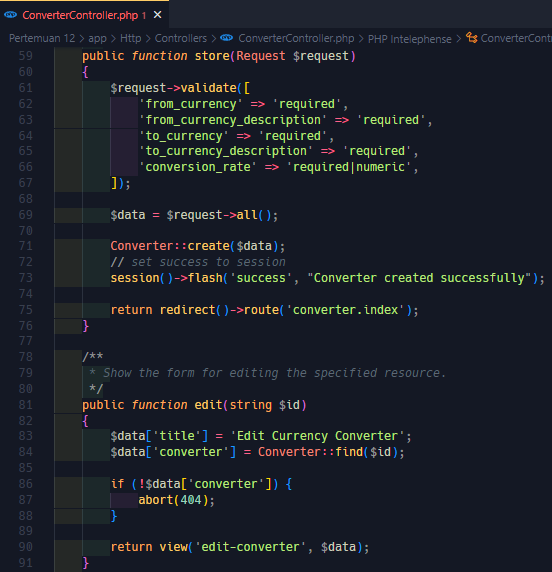
\includegraphics[width=0.6\textwidth]{classFiles/pertemuan-12-controller-part-3.png}
 \end{center}
\end{frame}

\begin{frame}[fragile]
 \frametitle{ConverterController.php Part 4}
 \vskip1cm
 \begin{center}
  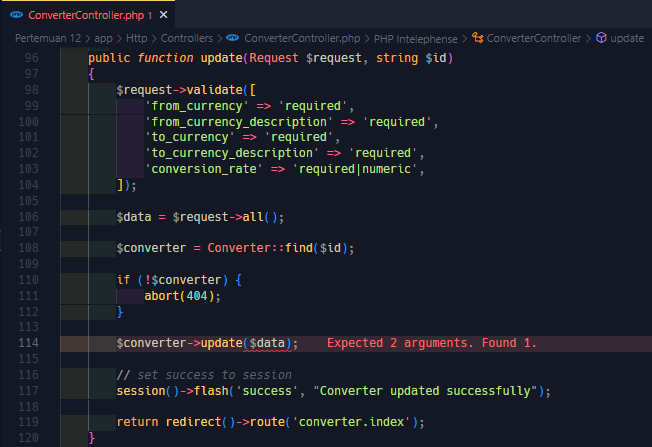
\includegraphics[width=0.6\textwidth]{classFiles/pertemuan-12-controller-part-4.png}
 \end{center}
\end{frame}

\begin{frame}[fragile]
 \frametitle{ConverterController.php Part 5}
 \vskip1cm
 \begin{center}
  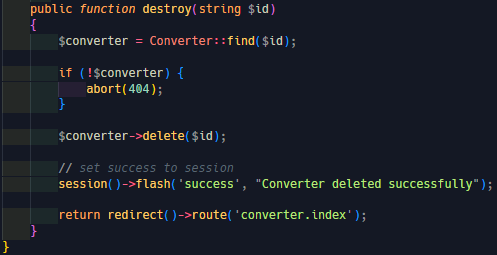
\includegraphics[width=0.6\textwidth]{classFiles/pertemuan-12-controller-part-5.png}
 \end{center}
\end{frame}

\begin{frame4}
    \frametitle{Thank You}
\end{frame4}

\end{document}
